\PassOptionsToPackage{unicode=true}{hyperref} % options for packages loaded elsewhere
\PassOptionsToPackage{hyphens}{url}
%
\documentclass[]{book}
\usepackage{lmodern}
\usepackage{amssymb,amsmath}
\usepackage{ifxetex,ifluatex}
\usepackage{fixltx2e} % provides \textsubscript
\ifnum 0\ifxetex 1\fi\ifluatex 1\fi=0 % if pdftex
  \usepackage[T1]{fontenc}
  \usepackage[utf8]{inputenc}
  \usepackage{textcomp} % provides euro and other symbols
\else % if luatex or xelatex
  \usepackage{unicode-math}
  \defaultfontfeatures{Ligatures=TeX,Scale=MatchLowercase}
\fi
% use upquote if available, for straight quotes in verbatim environments
\IfFileExists{upquote.sty}{\usepackage{upquote}}{}
% use microtype if available
\IfFileExists{microtype.sty}{%
\usepackage[]{microtype}
\UseMicrotypeSet[protrusion]{basicmath} % disable protrusion for tt fonts
}{}
\IfFileExists{parskip.sty}{%
\usepackage{parskip}
}{% else
\setlength{\parindent}{0pt}
\setlength{\parskip}{6pt plus 2pt minus 1pt}
}
\usepackage{hyperref}
\hypersetup{
            pdftitle={Learn R for Data Wrangling},
            pdfauthor={GA for TC},
            pdfborder={0 0 0},
            breaklinks=true}
\urlstyle{same}  % don't use monospace font for urls
\usepackage{longtable,booktabs}
% Fix footnotes in tables (requires footnote package)
\IfFileExists{footnote.sty}{\usepackage{footnote}\makesavenoteenv{longtable}}{}
\usepackage{graphicx,grffile}
\makeatletter
\def\maxwidth{\ifdim\Gin@nat@width>\linewidth\linewidth\else\Gin@nat@width\fi}
\def\maxheight{\ifdim\Gin@nat@height>\textheight\textheight\else\Gin@nat@height\fi}
\makeatother
% Scale images if necessary, so that they will not overflow the page
% margins by default, and it is still possible to overwrite the defaults
% using explicit options in \includegraphics[width, height, ...]{}
\setkeys{Gin}{width=\maxwidth,height=\maxheight,keepaspectratio}
\setlength{\emergencystretch}{3em}  % prevent overfull lines
\providecommand{\tightlist}{%
  \setlength{\itemsep}{0pt}\setlength{\parskip}{0pt}}
\setcounter{secnumdepth}{5}
% Redefines (sub)paragraphs to behave more like sections
\ifx\paragraph\undefined\else
\let\oldparagraph\paragraph
\renewcommand{\paragraph}[1]{\oldparagraph{#1}\mbox{}}
\fi
\ifx\subparagraph\undefined\else
\let\oldsubparagraph\subparagraph
\renewcommand{\subparagraph}[1]{\oldsubparagraph{#1}\mbox{}}
\fi

% set default figure placement to htbp
\makeatletter
\def\fps@figure{htbp}
\makeatother

\usepackage{booktabs}
\usepackage{amsthm}
\makeatletter
\def\thm@space@setup{%
  \thm@preskip=8pt plus 2pt minus 4pt
  \thm@postskip=\thm@preskip
}
\makeatother
\usepackage[]{natbib}
\bibliographystyle{apalike}

\title{Learn R for Data Wrangling}
\author{GA for TC}
\date{2020-04-28}

\begin{document}
\maketitle

{
\setcounter{tocdepth}{1}
\tableofcontents
}
\hypertarget{prerequisites}{%
\chapter{Prerequisites}\label{prerequisites}}

\hypertarget{what-to-expect}{%
\section{What to expect}\label{what-to-expect}}

This site will cover basic and intermediate topics in learning the use of R for \textbf{data wrangling} and visualization. This will serve as an introduction for data science. The basics of R and RStudio will be revisited, with some tips and tricks included, before moving on to using the Tidyverse library for manipulating, exploring and visualizing data.

The main tools that will be used are RStudio and the packages in the Tidyverse library, including dplyr, tidyr, ggplot2 and readr.

The general mode of operation will be to introduce R topics in sequence and to provide hand-picked apropriate online resources for those topics. However, some chapters, particularly the introductory ones, will have relatively extensive hand-written material. Other chapters might only provide summaries and supplementary comments to the provided online resources.

\hypertarget{resources-needed}{%
\section{Resources Needed:}\label{resources-needed}}

\begin{itemize}
\tightlist
\item
  R
\item
  RStudio
\item
  Web Browser
\end{itemize}

This tutorial assumes that R and RStudio have already been installed, but a link to installation instructions is provided.

\hypertarget{what-is-r}{%
\section{What is R?}\label{what-is-r}}

Such a simple question, but one worth answering. In short, the creators of the language originally defined it as `a programming language for data analysis and graphics' (Ihaka and Gentleman 1996). However, it has grown to much more than that. R can now be called \emph{a powerful integrated environment for statistical and data analysis, data processing, graphics and reporting}. R is \emph{open-source}, meaning that the R codebase is open to users, who can contribute to the development and improvement of the language, mainly through the creation of packages for different purposes and domains. This has led to an expansion of the use of R accross academia and the industry, with applications in official statistics, data science, machine-learning, web-scraping, interactive visualizations and more! R is a powerful tool that continues to improve and expand.

\hypertarget{is-it-worth-learning-r-for-data-wranglingdata-science-as-opposed-to-other-languages-like-python}{%
\section{Is it worth learning R for data wrangling/data science as opposed to other languages like Python?}\label{is-it-worth-learning-r-for-data-wranglingdata-science-as-opposed-to-other-languages-like-python}}

It is very much worth learning R. On the statistics side of things, R is used so extensively across academia because its tools and packages are very strongly developed and validated against standards for statistical practice and analysis.

\begin{quote}
``R is probably the most thoroughly validated statistics software on Earth.'' -- Uwe Ligges, CRAN maintainer (useR!2017).
\end{quote}

Therefore, for somebody that works in Official Statistics or academia, R is an easy choice. However, many people working in the industry or private sector prefer other tools such as Python, especially when it comes to data science and data analytics. Are these tools better than R? Not necessarily. Although all tools, softwares and languages have their pros and cons, R offers some very compelling advantages.

\textbf{Firstly}, R is more specialized. R was \emph{created} for statisitcal analysis and data manipulation. It was built by statisticians for statisticians and therefore considered the best language for statistical analysis and modeling. For example, R provides many easy ways to deal with missing values, and it has many well-built packages for survey data analysis. R is also believed to be the best language out there for data visualization through graphs, plots, etc.

\textbf{Secondly}, R has perhaps the best data-wrangling software on earth: Tidyverse. Tidyverse is a library containing a set of packages that vastly improve the data processing and data-wrangling capabalities of R. For example, it allows for easy reshaping, filtering, cleaning and querying of large datasets (dplyr and tidyr). It offers tools for quickly reading and writing files from different formats such as text, Excel, SPSS, STATA and more (readr package). Ggplot2 is perhaps the most popular graphing and visualization software there is, that allows plots and graphs to be build layer by layer in a very logical way.

\textbf{Third}, R has many other extended features that will help you in your data analysis workflow. Do you need to write a report with graphs, illustrations and tables? There is RMarkdown for that. Do you need an interactive website for running statistical models and visualizations? R Shiny was created for that purpose.

\textbf{All} of these advantages are unified by what is believed to be one of the best overall best programming IDE* out there: RStudio. RStudio is extremely powerful and flexible development environment, and it integrates all of what makes R so great. At the end of the day, it is all these advantages together that mmakes R such a commpelling sofware to learn.

That beig said, Python is considered to be better at general programming, machine learning and webscraping, and the data-science field on a whole leans more towards Python. However, R is still a major player in data science and it is absolutely worth learning data science with R. In addition, you will still be able to use Python modules and commands in R using the R Package `Reticulate'. Reticulate allows you to import and run Python code right in R. You can have the best of both worlds!

In conclusion, if you are a statistician or in academia, R is the way to go; and when you learn programming in R, you can apply these concepts later on in any other language, such as Python.

Now, let's take a look at starting to use R and RStudio.

*An IDE (Integrated Developoment Environment) is a program that provides many facilities for programmers to write, test and develop programs. It usually provides tools to manage the workflow and extensions to make coding easier. RStudio is considered by many the best IDE there is.

\hypertarget{intro}{%
\chapter{Introduction to R and RStudio}\label{intro}}

Now let us introduce the basic things needed for working with R: R and RStudio.

For an introduction of how to download R and how to install RStudio, please \href{https://cengel.github.io/R-intro/backgroud.html}{refer to this link}.

\hypertarget{the-rstudio-interface}{%
\section{The RStudio interface}\label{the-rstudio-interface}}

It will is useful to find a standard way to refer to the different parts of the RStudio interface. The following image uses the best naming convention I could find.

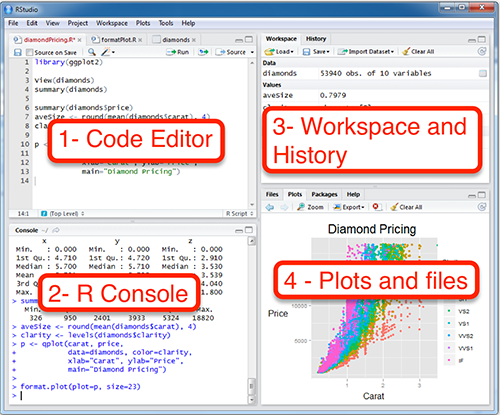
\includegraphics{images/rstudio-interface.png}

\hypertarget{the-code-editor}{%
\subsection{The Code Editor}\label{the-code-editor}}

Note that the upper-left pane is called the code editor. Although different people call it by different names, I think this one works best. Other terms for this part include ``source editor'' or ``script editor''.

This is basically where you will be doing all your typing and coding. To create a new R file or script, click on the first button on the top menu-bar and select, for example, new R script.

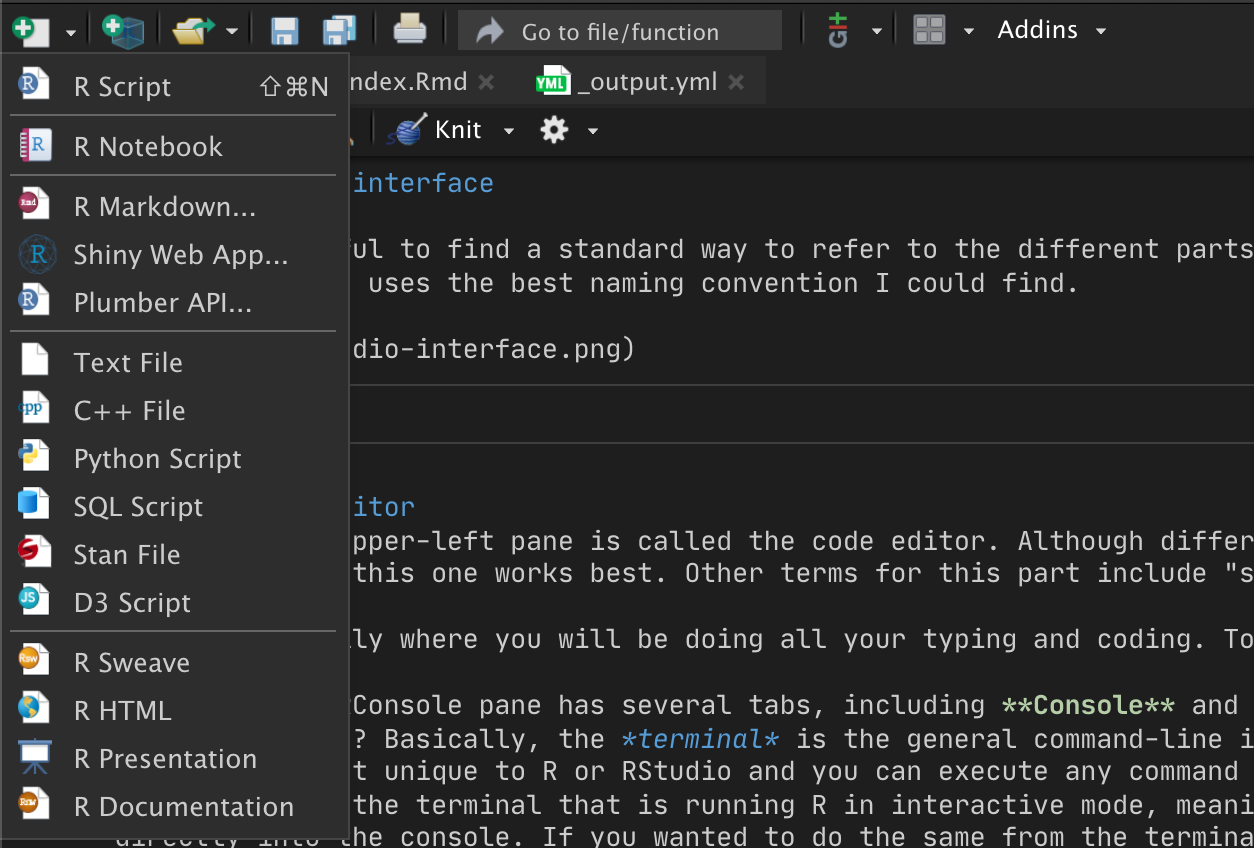
\includegraphics{images/new-rescript.png}

Once this new file is created, you can start writing your R code!

You can run all of the contents of an R script by clicking on the \textbf{Run} button in the top middle-right, or you can highlight a chunk of code in the code editor and press cmd+Enter to run that piece of code. This is very useful when testing a piece of code without having to run the entire script!


\includegraphics{images/run.png}

\hypertarget{the-r-console}{%
\subsection{The R Console}\label{the-r-console}}

The console is used to execute R code directly by typing R commands into it, and it also displays the results of the executed code. Whenever you execute any command from any other part of RStudio, the console will also produce some feedback. The console is basicaly ``R in interactive mode''.

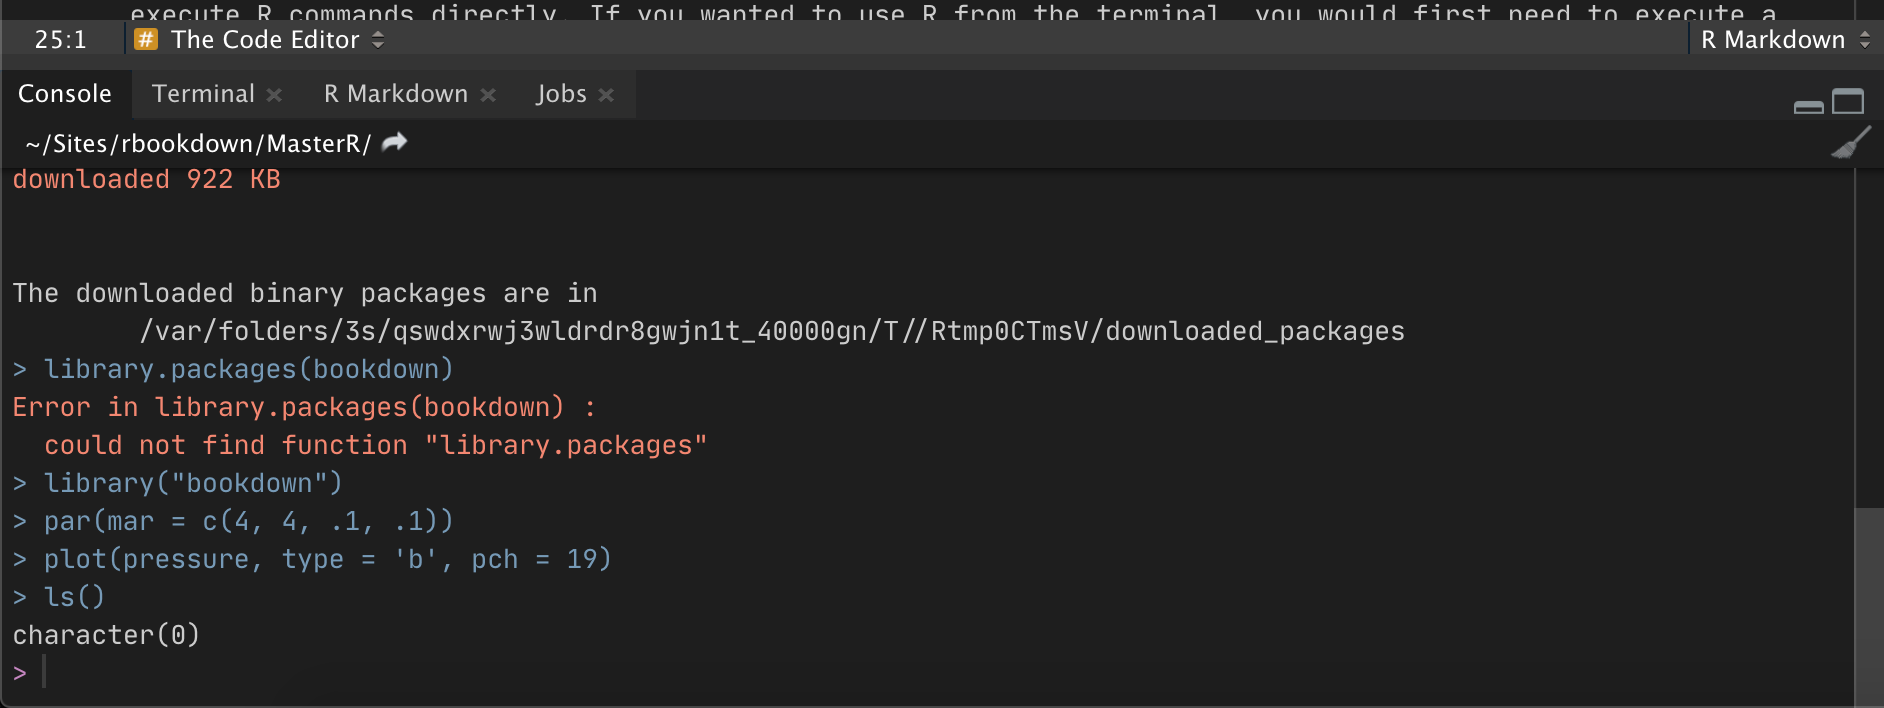
\includegraphics{images/console.png}

Note that the RConsole pane has several tabs, including \textbf{Console} and \textbf{Terminal}. What is the difference between the two? Basically,

\begin{itemize}
\item
  The \emph{terminal} is a general command-line interface that all computers have. It is used for executing commands of many types and is not unique to R or RStudio.
\item
  The \emph{Console} is a \textbf{subset} of the terminal that is running R in interactive mode, which allows you execute R commands directly. If you wanted to use R from the terminal, you would first need to execute a separate command to call and initiate R.
\end{itemize}

\hypertarget{the-workspace-and-history-pane}{%
\subsection{The Workspace and History pane}\label{the-workspace-and-history-pane}}

This pane gives you an overview of your \textbf{working environment}. For one, it tells you how many variables and data objects you currently have loaded into memory. You can click on data objects (such as tables) to view the contents. This is very useful when you import files and save them into R objects. Here is an example of a workspace with some data and variables (\emph{values}) loaded.

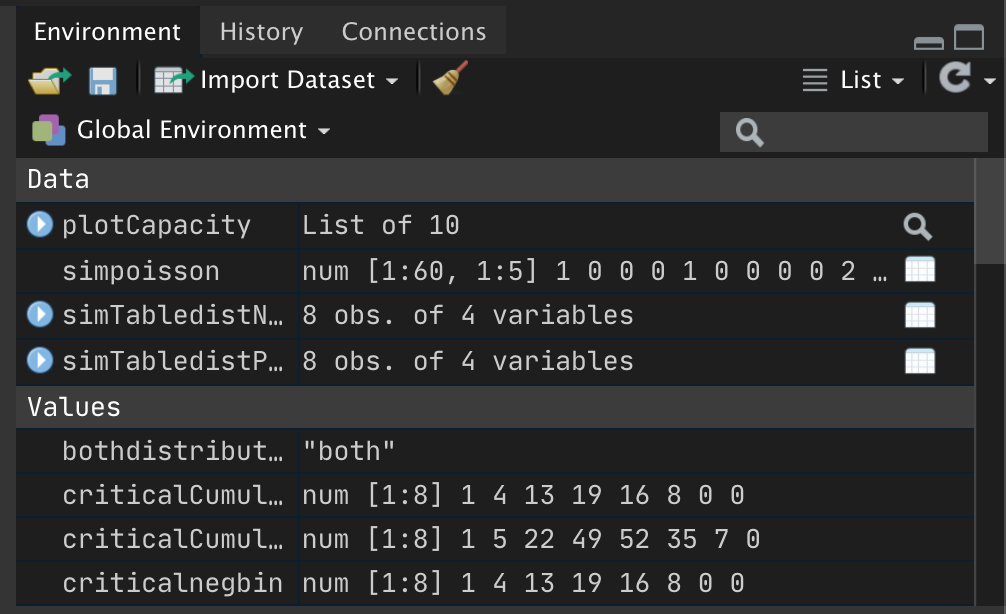
\includegraphics{images/workspace.png}

To see on the console all the R objects currently loaded into your R Workspace, use the ls() command

\begin{verbatim}
ls()
\end{verbatim}

To remove objects from memory, use the rm() command:

\begin{verbatim}
#removes all objects
rm(list = ls())

#removes one object
rm(object_name)

#removes multiple objects
rm(c("object1", "object2", "object3"))
\end{verbatim}

You can also save the current state of your working environment (all objects etc) so that if you close RStudio and then later you open it again, you can pick up where you left off. To do this:

\begin{verbatim}
# save all items in workspace to a .RData file 
save.image()

# save specified objects to a .RData file 
save(object1, object2, file = "myfile.RData") 

# load workspace into current session
load("myfile.RData")
\end{verbatim}

\textbf{\emph{However}}, you don't really have to this manually as RStudio automatically asks you if you want to save your workspace, and then it reloads the previously saved workspace whenever you open the project again.

\hypertarget{the-file-and-plots-or-miscellaneous-pane}{%
\subsection{The File and Plots (or Miscellaneous) pane}\label{the-file-and-plots-or-miscellaneous-pane}}

The bottom right pane contains multiple tabs. The Files tab allows you to see which files are available in your working directory. The Plots tab will display any visualizations that are produced by your code. The Packages tab will list all pack- ages downloaded to your computer and also the ones that are loaded (more on this concept of packages shortly). And the Help tab allows you to search for topics you need help on and will also display any help responses (more on this later as well).

\hypertarget{the-working-directory}{%
\section{The working directory}\label{the-working-directory}}

Whenever you create a new project, RStudio automatically sets your \textbf{working directory} to that specific folder where you created the project.

What is the working directory and why is it important?

The working directory (wd) is, essentially, the point of reference for the particular project you are working on. The Files pane in RStudio (lower-right pane) will display the files and folders in your current wd. And wenever you want to refer to external files in your R code, your wd will once more be your point of reference and you can use \emph{relative} file-paths (relative to the wd), as opposed to absolute file paths (would need to type the entire path).

For example, lets say you create a new project called \emph{DataWrangling}. And in there, you create an RScript called script.R; this is where you are writing your R code. Now lets say you have a CSV file called meals.csv where you are keeping a meal schedule, and you want to manipulate some of that data in R. Well, if you copy the meals.csv file to your working directory, you can access that file using a \textbf{relative path}. For example, to store the contents of the file you would be able to use a command like the following:

\begin{verbatim}
mealsFrameRelative <- read.csv('meals.csv')
\end{verbatim}

The absolute path for the file would look like this (see how much longer it is):

\begin{verbatim}
mealsFrameAbsolute <- read.csv('Users/gian/sites/R/DataWrangling/meals.csv')
\end{verbatim}

In order to see your current working directory, use getwd():

\begin{verbatim}
getwd()
\end{verbatim}

To change it to somewhere else, use setwd():

\begin{verbatim}
setwd('path/to/new/directory')
\end{verbatim}

The main thing to remember is: each project will have its own working directory, usually the folder where you created the project, but this can be changed with setwd().

If you have a Mac, I suggest that you keep your R projects under User \textgreater{} Sites \textgreater{} R \textgreater{} {[}ProjectName{]}

For example, here I have a few projects under my Sites \textgreater{} R directory: 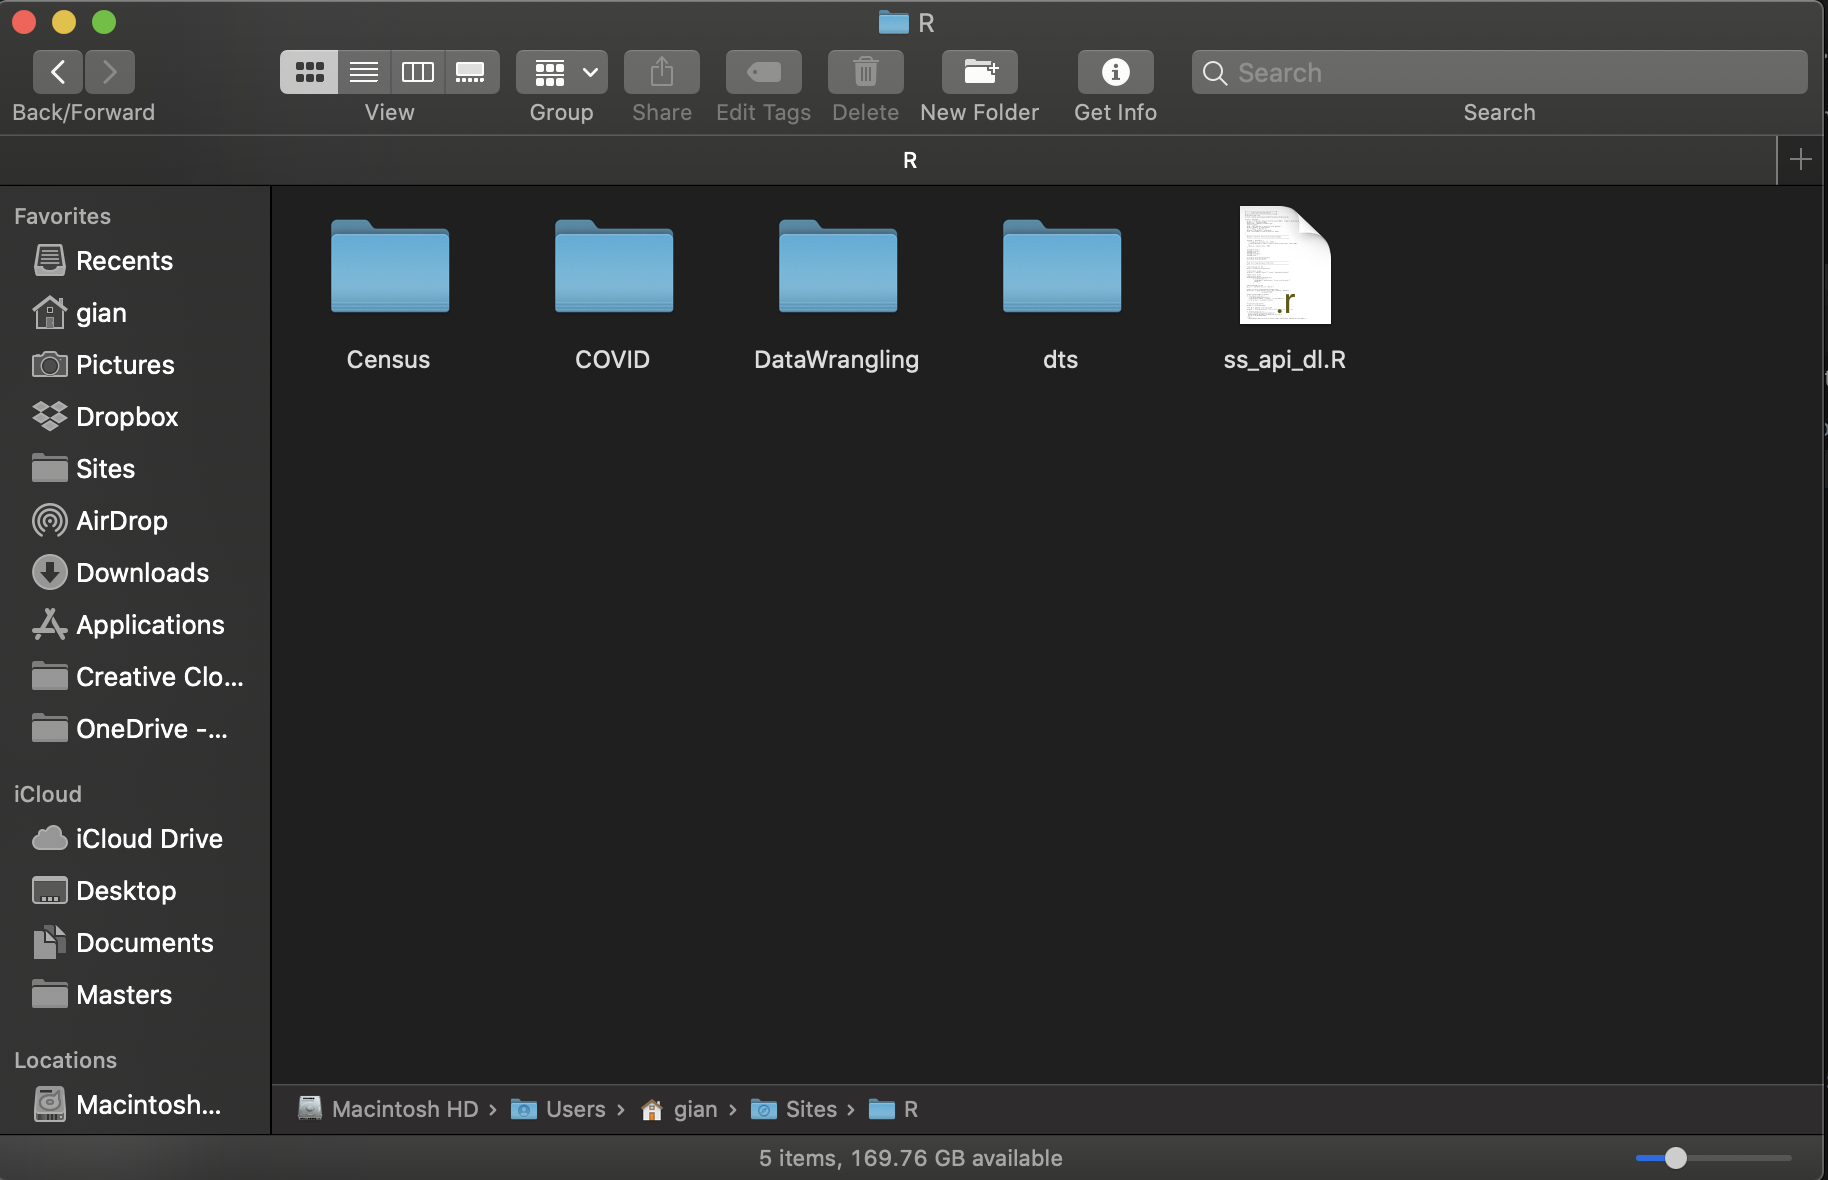
\includegraphics{images/wd.png}

\hypertarget{r-and-rstudio-tips}{%
\section{R and RStudio tips}\label{r-and-rstudio-tips}}

\hypertarget{organizing-your-working-directory}{%
\subsection{Organizing your working directory}\label{organizing-your-working-directory}}

Usually, when you start an R projects, you will be working with a variety of different files, often of different types. For example, you have your R scripts which end with the file extension \emph{.R}. You also likely will use data files such as CSV or Excel or SPSS files. If you write reports, you will also likely have PDF and Word files. A good way to organize all of these files in a logical manner is to, inside of your working directory, create the following folders:

\begin{itemize}
\tightlist
\item
  \textbf{scripts} - to keep your .R and .RMd (markdown) files.
\item
  \textbf{data} - to keep all your data files that you will use to work with.
\item
  \textbf{reports} - to keep your output documents and reports.
\end{itemize}

This is how it would look in practice, if I have a project called \emph{DataWrangling} and I have the previously mentioned folder structure: 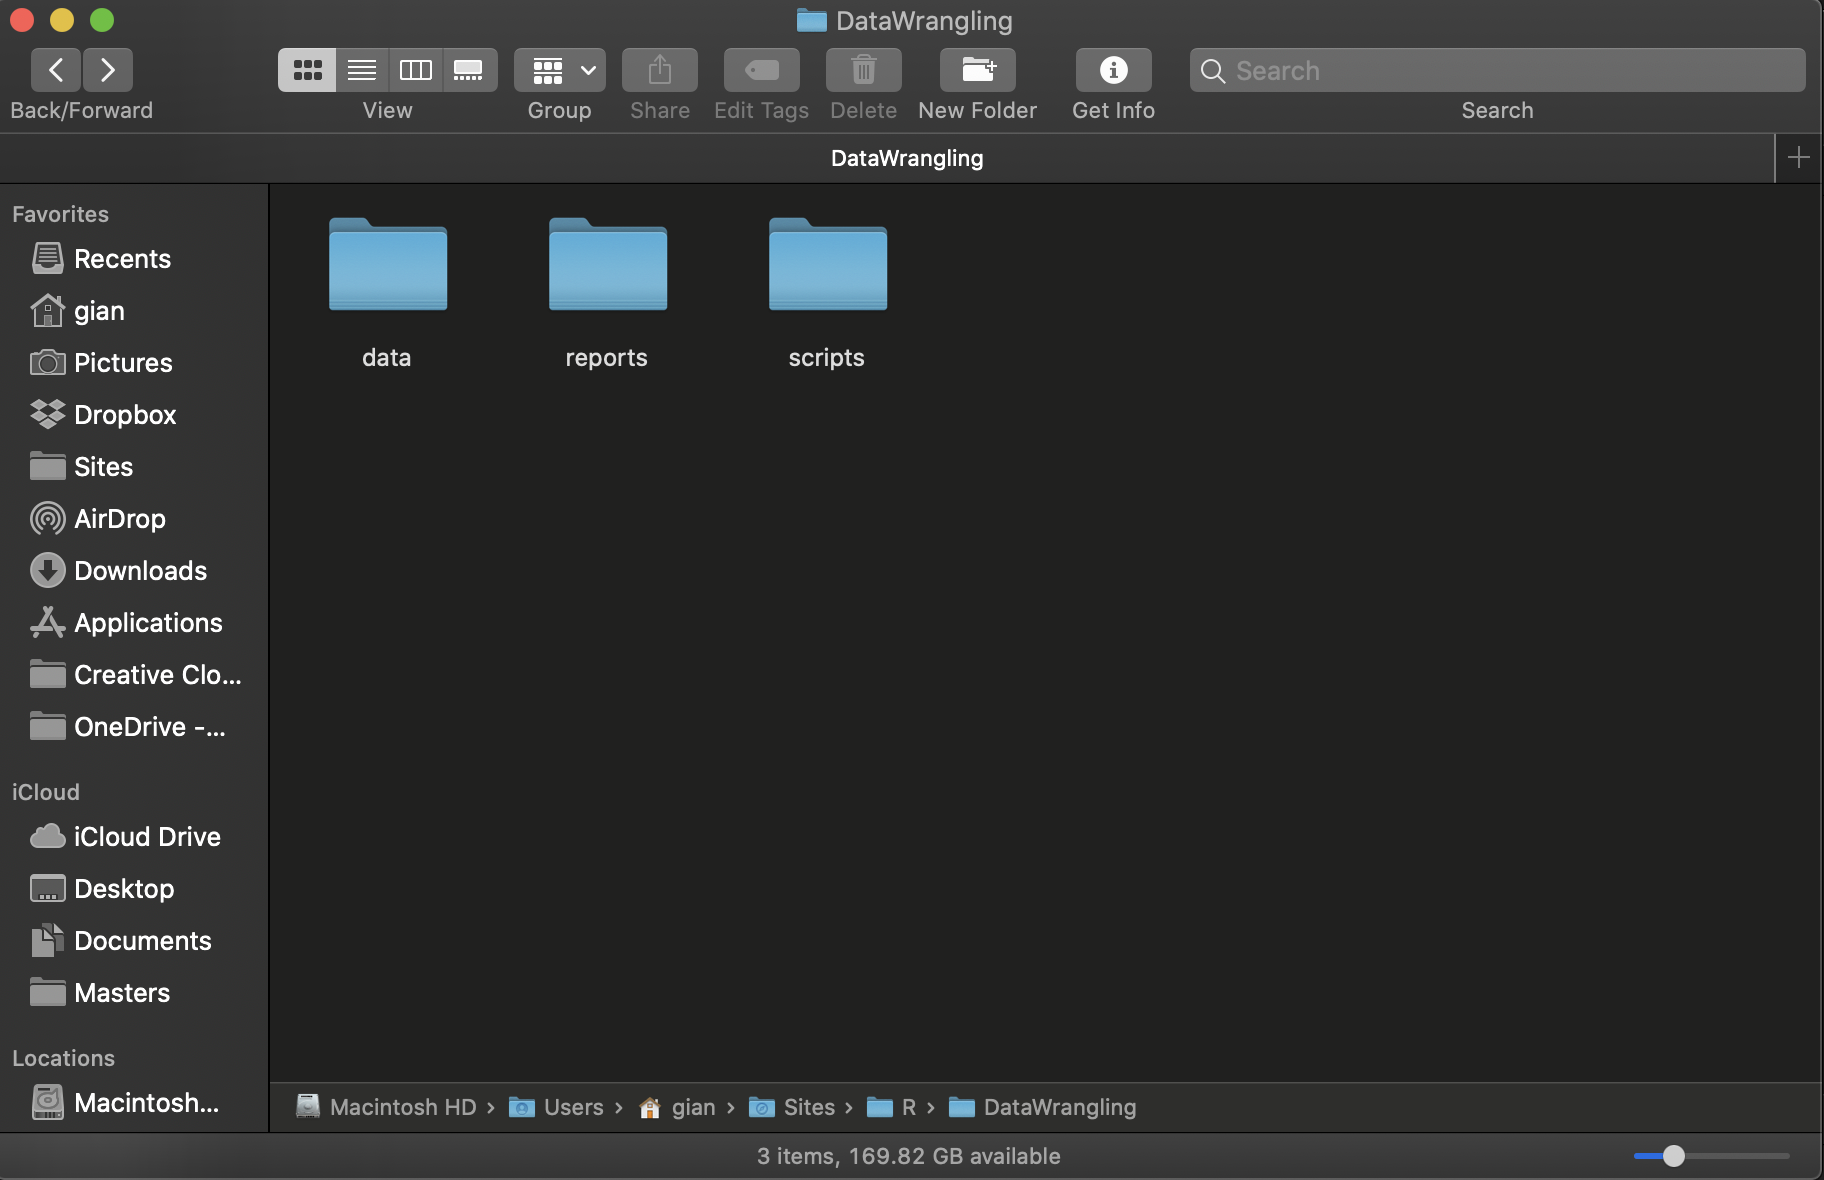
\includegraphics{images/structure.png}

\hypertarget{other-ways-to-use-r}{%
\subsection{Other ways to use R}\label{other-ways-to-use-r}}

Even though RStudio is the main and preferred way to interact with R, it is not the only way.

Once R is installed, it can be run from the Mac/Windows terminal using the command \emph{R}, which will trigger the interactive mode and you will be able to type R commands. This is useful to remember because you can also type

\begin{verbatim}
R myScript.R
\end{verbatim}

From the terminal and it will automatically execute whatever code you have in the file called myScript.R. In the programming world, we call this \emph{working from the command line} (meaning, working without an interface, directly into the terminal or console).

Also remember, to write R code (or any programming language), all you need is a text editor. You don't need to use RStudio to write R, although it is preferred, and you can view/edit R files with the default text editor, or more specialized coding-oriented text editors such as \href{https://code.visualstudio.com}{VS Code}. Whatever you use to write R code, you can later open it and edit it with RStudio if you prefer. This is a useful tip if you ever have to write R in a computer that does not have RStudio installed. Just remember to save the file with the \emph{.R} extension.

\hypertarget{r-language-basics}{%
\chapter{R Language Basics}\label{r-language-basics}}

\hypertarget{objectives}{%
\section{Objectives}\label{objectives}}

\begin{enumerate}
\def\labelenumi{\arabic{enumi}.}
\tightlist
\item
  To get a refresher on the basics of R programming.
\item
  To understand objects and functions.
\item
  Learn how to create and use vectors.
\item
  Learn how to deal with missing data.
\item
  Learn how to use the help and documentation.
\end{enumerate}

\hypertarget{glossary-of-terms}{%
\section{Glossary of terms}\label{glossary-of-terms}}

\begin{itemize}
\tightlist
\item
  \textbf{Project}: An R project consisting of a main folder (as the working directory), and all the files within.
\item
  \textbf{Object}: An R variable. This can be a single value, a vector, list, matrix, data frame or other. Almost everything in R is referred to as an object, though there are several types of objects.
\item
  \textbf{Function}: A command in R that executes a specific action and usually returns a value. For example, the \texttt{sum()} function usually takes values for addition as arguments, and returns the sum.
\item
  \textbf{Arguments}: These are values or inputs passed into functions. For example in the function \texttt{sum(a,\ b)}, a and b are \emph{arguments} to the sum function. These will be added and the sum will be returned. Functions usually have documentation where they specify which arguments are required for the function to work properly.
\item
  \textbf{Package}: A package, sometimes called a \textbf{library}, is a set of related pre-created functions in R. It is code that has been written by other people and then packaged together so that others can download the code and re-use it. For example, if somebody were to write code about how to simulate and model the behavior of an epidemic or infectious disease, they could create a package with the related code and documentation, so that others can benefit and use it as well.
\end{itemize}

\hypertarget{creating-a-new-r-project}{%
\section{Creating a new R project}\label{creating-a-new-r-project}}

To start, lets create a new project in R and call it DataWrangling. As mentioned, it is recommended to create this project in the directory \texttt{user/sites/R/}.

Click on the \emph{File \textgreater{} New Project} and then select \emph{New Directory \textgreater{} New Project \textgreater{} {[}Select directory and enter project name{]} \textgreater{} Create}.

Once the project is created, create a new R script by going to \emph{File \textgreater{} New File \textgreater{} R Script}.

\hypertarget{getting-started-with-code}{%
\section{Getting started with code}\label{getting-started-with-code}}

\hypertarget{creating-objects}{%
\subsection{Creating objects}\label{creating-objects}}

For the purpose of learning the basics of R coding, we will refer to this \href{https://cengel.github.io/R-intro/gettingstarted.html}{excellent online resource}. In addition to that, I will provide a summmary of the important points.

\hypertarget{objects-and-assignment-of-values}{%
\section{Objects and assignment of values}\label{objects-and-assignment-of-values}}

To create an objects and assign values:

\begin{verbatim}
object1 <- 5
object2 <- 10

object3 <- object1 + object2
\end{verbatim}

\hypertarget{which-assignment-operator-to-use}{%
\subsection{Which assignment operator to use}\label{which-assignment-operator-to-use}}

The traditional assignment operator in R is the left-facing arrow \texttt{\textless{}-}. With time, the language also evolved to use the equal-sign \texttt{=} for this same purpoose. However, the standard practice is to always use the arrow operator \texttt{\textless{}-} for assigning values to objects, and to use the equal sign \texttt{=} to specify function arguments. For example:

\begin{verbatim}
newPerson <- createNewPerson(name = "John Doe", age = 45)
\end{verbatim}

In the previous example, the function \texttt{createNewPerson()} is called and two arguments (\texttt{name} and \texttt{age}) are provided. The result of the function is then assigned to the object \texttt{newPerson}. Note that the values provided to the arguments were specified using the equal-sign \texttt{=} while the assignment of the resulting value to the newPerson object was donw with the assignmment arrow operator \texttt{\textless{}-}.

\textbf{Tip}: Use \texttt{option} + \texttt{-} in Mac or \texttt{alt} + \texttt{-} in PC and RStudio will type in the arrow operator for you. This is very convenient and saves time and keystrokes.

\hypertarget{comments}{%
\section{Comments}\label{comments}}

Use the pound or hash sign \texttt{\#} to write comments in your code. Comments are non-executable pieces of writing that help explain your code.

Sometimes, it is useful to ``comment out'' R code that is not currently being used, or when you want intend to delete a piece of code but are not sure yet if it is the write decision. You can add \# to the beginning of each line of code that you want to be skipped during execution.

\textbf{Tip}: To comment out large chunks of code at a time, select/highlight the code and then use \texttt{commmand} + \texttt{shift} + c (or \texttt{ctrl} + \texttt{shift} + c in Windows). Select the same code and press the same sequence of keys to un-comment the code later, if necessary.

\hypertarget{functions-and-arguments}{%
\section{Functions and arguments}\label{functions-and-arguments}}

A function takes inputs and returns a value - the result of the function. A function executes pre-written commands using the arguments (inputs) provided, and returns the result. For example executing the code \texttt{sum(1,3,5)} will return the value \texttt{9}.

Many functions have arguments that need to be provided explicitly. For example, the following function:

\begin{verbatim}
createNewPerson(name = "John Doe", age = 45)
\end{verbatim}

Has two arguments that must be explicitly specified (written out) when \_\_calling*\_\_ the function.

*Calling a function is the term used when a function is executed in the code.

\hypertarget{types-of-objects}{%
\section{Types of objects}\label{types-of-objects}}

\hypertarget{vectors}{%
\subsection{Vectors}\label{vectors}}

Vectors are the most common type of object in R, and consist of a group or sequence of values (in other programming languages, vectors are called `arrays'). A vector is defined using the c() function. For example:

\begin{verbatim}
ageVector <- c(19,22,20,18,18,19,22,21)
\end{verbatim}

In the previous code, I created a vector called ageVector by using the c() function to combine a group of values into a vector.

There are several R functions that help you get information on vectors (and other objects), such as:

\begin{itemize}
\tightlist
\item
  \texttt{length()}: Tells you the number of elements (distinct values) in the vector.
\item
  \texttt{class()}: The type of data contained in the vector (such as numeric or string/character)
\item
  \texttt{str()}: Detailed information about the structure and contents of the vector, including length and class, but other details as well.
\end{itemize}

\hypertarget{subsetting-vectors}{%
\subsubsection{Subsetting vectors}\label{subsetting-vectors}}

Subset vectors by using brackets {[}{]} after the object name and then specifying the index of the element/value you are interested in.

\begin{verbatim}
ageVector[1]
\end{verbatim}

Returns the first value in the vector.

\begin{verbatim}
ageVector[c(1,2,4)]
\end{verbatim}

Returns the first, second and fourth values.

\begin{verbatim}
ageVector[-1]
\end{verbatim}

Returns all values \emph{except} the first.

\begin{verbatim}
ageVector[-c(1,3,5)]
\end{verbatim}

Returns all values \emph{except} the first, third and firth values.

\begin{verbatim}
ageVector[2:5]
\end{verbatim}

Returns all values between the second and fifth, inclusive.

\hypertarget{matrix}{%
\subsection{Matrix}\label{matrix}}

A matrix consists of rows and columns. All columns must be of the same length as well as all rows (Eg: cant have a row with 3 entries and another with 5). To construct a matrix, we use a function conveniently called matrix().

\texttt{y\ \textless{}-\ matrix(1:20,\ nrow=5,ncol=4)\ \#\ generates\ 5\ x\ 4\ numeric\ matrix}

Subset a matrix with {[}row , column{]}:

\begin{verbatim}
y[,4]       # 4th column of matrix
y[3,]       # 3rd row of matrix
y[2:4,1:3]  # rows 2,3,4 of columns 1,2,3
\end{verbatim}

\hypertarget{list}{%
\subsection{List}\label{list}}

Lists can have elements of any type and length. To construct one, use the list() function:

\begin{verbatim}
myl <- list(id="ID_1", a_vector=animals, a_matrix=y, age=5.3) # example of a list with 4 components
myl[[2]] # 2nd component of the list
myl[["id"]] # component named id in list
\end{verbatim}

\hypertarget{data-frame}{%
\subsection{Data frame}\label{data-frame}}

Data frames in R is like a mixture of lists and matrices. You have a set named columns each of which can be of different type (like in a list), but all columns must be of same length (like in a matrix). A way to think about a data frame is like a table in Excel and is commonly used to store tabular-type data.

Here is how you could construct a data frame.

\begin{verbatim}
mydf <- data.frame(ID=c(1:4),
                   Color=c("red", "white", "red", NA),
                   Passed=c(TRUE,TRUE,TRUE,FALSE),
                   Weight=c(99, 54, 85, 70),
                   Height=c(1.78, 1.67, 1.82, 1.59))

mydf
\end{verbatim}

\hypertarget{missing-data}{%
\section{Missing data}\label{missing-data}}

R automatically codes missing data with the \texttt{NA} value. Datasets that have missing data can be processed with a variety of ways that will help you decide how to deal with these missing values. Dealing with missing values is important when operating with rows and columns of data. For example, you might want to add all values in a row to get a total, but what happens if you have a bunch of NAs?

There are two main ways:

\begin{enumerate}
\def\labelenumi{\arabic{enumi}.}
\tightlist
\item
  Using the \textbf{na.rm} argument. Many functions such as sum() and mean() have an argument called \textbf{na.rm} (basically: NA remove) which you can set to TRUE in order to ignore missing values. For example:
\end{enumerate}

\begin{verbatim}
heightVector <- c(110, 120, NA, NA, 100, NA)

avgHeight <- mean(heightVector, na.rm = TRUE)
\end{verbatim}

\begin{enumerate}
\def\labelenumi{\arabic{enumi}.}
\setcounter{enumi}{1}
\tightlist
\item
  Use functions such as \texttt{na.omit()} or \texttt{is.na()}. For example:
\end{enumerate}

\begin{verbatim}
heightVector <- c(110, 120, NA, NA, 100, NA)

avgHeight <- mean(na.omit(heightVector))
\end{verbatim}

or

\begin{verbatim}
heightVector <- c(110, 120, NA, NA, 100, NA)

avgHeight <- mean(!is.na(heightVector))
\end{verbatim}

Note the exlamation point before !is.na(), which makes sure that the function returns the values that are \textbf{not} NA. Otherwise, is.na() returns values that \textbf{are} NA. The exclamation point negates or reverses the operation.

\hypertarget{help-and-documentation}{%
\section{Help and documentation}\label{help-and-documentation}}

For general R help, look at the `Help' tab in the Files and Miscellaneous pane.
For quick help relating to any function or package, use the question mark \texttt{?} before the name of a function or package.

\begin{verbatim}
?sum
\end{verbatim}

Will open up the documentation for the sum() function and tell you how to use it.

\hypertarget{extra-topic-naming-and-notation}{%
\section{Extra topic: Naming and notation}\label{extra-topic-naming-and-notation}}

Objects or variables can have practically any namme, but there are some rules:

\begin{enumerate}
\def\labelenumi{\arabic{enumi}.}
\tightlist
\item
  Cannot start with a number, but can have numbers in the name.

  \begin{itemize}
  \tightlist
  \item
    \texttt{1time} is not valid, but \texttt{time1} and \texttt{time1result} are valid.
  \end{itemize}
\item
  Cannot be one of key-words or reserved words in R. For example, terms such as \texttt{if}, \texttt{else}, \texttt{for}, and \texttt{function} already have specific uses in R and cannot be used for names of objects.
\item
  Must be descriptive, but succint.
\item
  Are case sensitive: \texttt{value1} is not the same as \texttt{Value1}, these are different objects.
\end{enumerate}

In addition, there are several styles for naming and writing object names, especially if the name consists of more than one ``English'' word. For example, I previously referred to an object called \texttt{newPerson}. A different programmer maybe would have preferred to name it \texttt{new\_person} instead. This is what we refer to when we talk about naming-styles or naming-conventions. The main styles are as follows:

\begin{itemize}
\tightlist
\item
  Camel-case: the first word is small-letters, but all other words start with a capital letter.

  \begin{itemize}
  \tightlist
  \item
    Eg: \texttt{newPerson}, \texttt{verySmallChild}, \texttt{totalSum}.
  \end{itemize}
\item
  Underscore sepatator: Uses underscores \texttt{\_} to separate the words.

  \begin{itemize}
  \tightlist
  \item
    Eg: \texttt{new\_person}, \texttt{very\_small\_child}, \texttt{total\_sum}.
  \end{itemize}
\item
  All small: The entire name is in small letters.

  \begin{itemize}
  \tightlist
  \item
    Eg; \texttt{newperson}, \texttt{verysmallchild}, \texttt{totalsum}.
  \end{itemize}
\end{itemize}

The important thing about notation styling is to just be consistent. I personally preferr to use \texttt{camelCase} for object and variable notation in programming language. However, when working with databases and the SQL language, it is recommended to use \texttt{underscore\_separators} to name your tables and table-fields (columns). Therefore, when creating tables (or data frames) in R, I will typically use \texttt{underscore\_separators} when naming the columns; but I will use \texttt{camelCase} for the names of any other kind of object. Eg:

\begin{verbatim}
salesTable <- data.table(value_one, value_two, total_sales)
\end{verbatim}

The previous example is not really valid R code, but it illustrates the naming convention principles that were previously discussed.

\hypertarget{challenge}{%
\section{Challenge}\label{challenge}}

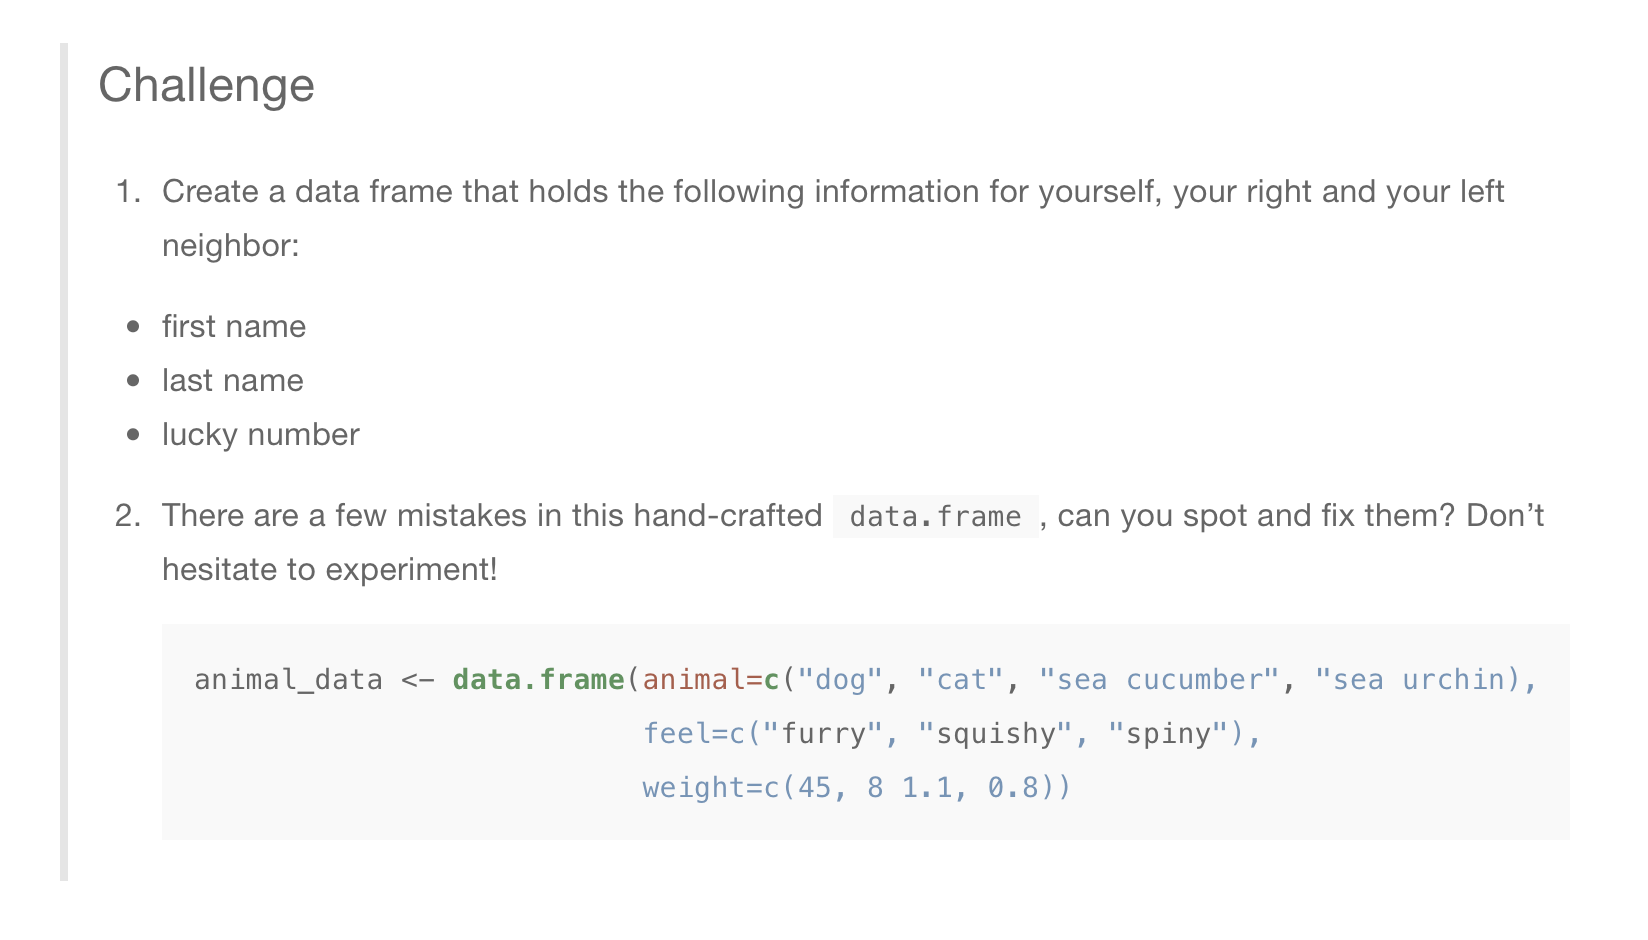
\includegraphics{images/challenge1.png}

\bibliography{book.bib,packages.bib}

\end{document}
